\documentclass[12pt]{article}

\usepackage{hyperref} %links in ToC
\usepackage{caption} %interesting things with captions
\usepackage[margin=1.5in]{geometry} %mostly set margin of the report
\usepackage{tabulary} %text wrapping in tables
\usepackage{subcaption} %let me put multiple images into a single caption

%images being embeded
\usepackage{graphicx}
\graphicspath{ {images/} }

%code highlighting
\usepackage{minted}
\setminted[c++]{frame=single,linenos=true,autogobble=true,numbersep=4pt,tabsize=4}
\setminted[bash]{frame=single,linenos=true,autogobble=true,numbersep=4pt,tabsize=4}
\setminted[xml]{frame=single,linenos=true,autogobble=true,numbersep=4pt,tabsize=4}

%fix a quote mark issue
\usepackage [english]{babel}
\usepackage [autostyle, english = american]{csquotes}
\MakeOuterQuote{"}


\begin{document}
\pagenumbering{gobble}
\begin{titlepage}
	\centering
	{\Huge Virtualisation\par}
	\vspace{0.25in}
	{\Large Project 1\par}
	\vspace{2in}
	{Alex Harper\par}
	\newpage
\end{titlepage}
\pagenumbering{roman}

\tableofcontents
\newpage

\listoffigures
% \listoftables
\newpage
\setlength{\parindent}{4em} %indent of first line of paragraph
\setlength{\parskip}{1em} %space between paragraphs

\pagenumbering{arabic}

\section{Introduction}

Reading through the book, I am not sure what I am supposed to write about.
The book itself is fairly comprehensive so all i can think of is me screwing aroudn with some minor things and write about it here.
I have been using virtual machines for awhile now, mostly to mess with soemthing and then trow away the VM or to have a working install of windows.
The sections i write about are generally about specifics around virtual machines, things that I had questions myself and decided to look up.

\section{Networking}

Without the internet, computers are limited in usefulness these days.
To augment what is in the book, I talk about the specific types of virtual networks that I have available on my system.
The table fig\ref{fig:network_type_table} show the list and a quick description of connection type and table fig\ref{fig:network_device_table} shows the different devices the NIC is emulated as.

The type of network makes a difference for what you are trying to do, each type of connection having limitations to them.
The \textit{macvtap} and \textit{bridge} connections allow a VM to act like it is directly on the network, almost directly sending packets on the hardware.
The drawback is that it does not allow Host - Guest communication.
The \textit{NAT} types of connections allow network access also, but they do not direclty expose the VM to the netowrk.
This is fine for outgoing connections but to host something on the VM, port forwarding must be setup to expose the service.
This apparently does allow Host - Guest communication but only by sending to the adapter itself to just have it return it. (aka, can't use the loopback because firewall rules)
The \textit{Internal Network} only allows inter-VM communication.
This is good if you wanted to seperate services to different VMs but the services (like a database) does not need internet access.
The \textit{Host Only} connection creates a local connection to the host with its own ip range.
Using system firewall rules, you can get everything to work through this, but is only meant for local availability (aka only Host-Guest).

The different hardware listed in fig\ref{fig:network_device_table} has several options.
I have not been able to find any difference in them, etiehr speed or features, so I just leave it with the default.

\begin{figure}[ht]
	\centering
	\begin{tabular}{|l|l|p{0.6\textwidth}|}
	\hline
	Type & System & Description \\ \hline
	macvtap & KVM & Impersonates a different MAC address directly on the physical NIC \\ \hline
	NAT & BOTH & Assigns an address to the VM and provides internet access \\ \hline
	NAT Network & VBox & Same as NAT but is a virtual network so allows inter-guest comunications \\ \hline
	Bridge & VBox & Seems to be similar to macvtap \\ \hline
	Internal Network & VBox & Makes a virtual network that VMs can communicate over but does not providde external network access \\ \hline
	Host Only & VBox & Single connection to the host only, allowing the VM-Host communication but not network access \\ \hline
	\end{tabular}
	\caption{Quick Reference of Networking Types}
	\label{fig:network_type_table}
\end{figure}

\begin{figure}[ht]
	\centering
	\begin{tabular}{|l|l|}
	\hline
	Type & System \\ \hline
	rtl8139 &KVM \\ \hline
	e1000 &KVM \\ \hline
	virtio &Both \\ \hline
	Intel Pro/1000 MT desktop &VBox \\ \hline
	Intel Pro/1000 T server &VBox \\ \hline
	Intel Pro/1000 MT server &VBox \\ \hline
	PCnet-PCI II &VBox \\ \hline
	PCnet-FAST III &VBox \\ \hline
	\end{tabular}
	\caption{Quick Reference of Networking Devices}
	\label{fig:network_device_table}
\end{figure}

The various connections is interesting for their limitations, but lets look at performance.
The first tool people really learn about for netowrking is \textit{ping}.
Besides just return time, I also tested the throughput by copying a 10gig file over from my NAS to the VM.
Below in fig\ref{fig:performance_network} are the various metrics I recorded for the different connections.
The Host to NAS connection is saturationg the gigabit connection and the NAS can probably go faster if the network allowed.
The KVM to Host connection seemed to be bottlenecking at the CPU level in the VM.

\begin{figure}[ht]
	\centering
	\begin{tabular}{|l|l|l|l|}
	\hline
	&& Ping & Speed \\ \hline
	Host to Router & & 0.38 ms & --- \\ \hline
	Host to NAS & & 0.28 ms & 118 MB/s \\ \hline
	VBox to NAS & Bridge & 0.478 ms & 27 MB/s \\ \hline
	VBox to Host & NAT & 0.17 ms & 32 MB/s \\ \hline
	VBox to Host & Host-Only & 0.18 ms & 44 MB/s\\ \hline
	KVM to NAS & macvtap & 0.393 ms & 53 MB/s \\ \hline
	KVM to Host & NAT & 0.095 ms & 3 MB/s \\ \hline
	\end{tabular}
	\caption{Performance Metrics}
	\label{fig:performance_network}
\end{figure}

\section{Backing Filesystem}

There are two ways to think about what this is talking about; what file are we using for the virtual disk, and what file system is that file saved on.

\subsection{RAID}

The book mentions RAID as a means of increasing availability but does not seem to go deep into what it is really about.
RAID is the acronym standing for \textbf{R}edundent \textbf{A}rray of \textbf{I}nexpensive \textbf{D}isks.
The original idea was to use a set of disks for different tasks that different work loads would benifit from.
There are different "levels" of RAID, each with a certain meaning of configuration for how the data is distributed.
Below is a quick reference table of the different levels int fig\ref{fig:raid_levels} (source \cite{wiki_raidLevels}).

\begin{figure}[ht]
	\centering
	\begin{tabular}{|c|p{0.8\textwidth}|}
	\hline
	0 & Disks are transparently appended so appears the size of all the disks added together (Similar to JBOD) but the data is stripped \\ \hline
	1 & Each disk is a simple copy of all the other disks \\ \hline
	2 & Deprecated - Stripes data across multiple disks at the bit level \\ \hline
	3 & Deprecated - Stripped data at the byte level with a sinlge disk used for parity \\ \hline
	4 & Deprecated - Stripped data at the block level with a single disk used for parity \\ \hline
	5 & Stripped data at the block level with parity blocks evenly distributed across all the disks \\ \hline
	6 & Same as RAID5 but 2 parity blocks per block level \\ \hline
	\end{tabular}
	\caption{RAID Levels}
	\label{fig:raid_levels}
\end{figure}

It is interesting to see that the earliest (and simplest) levels are still used, while the more complicated versions had to be replaced.
The levels 0 and 1 are still used frequently today because of the performance they provide.
Levels 2, 3, and 4 had neat ideas, but due to limitations and changes in computing, they got supercedded by levels 5 and 6.
5 and 6 tooks ideas and lessons learned from the other levels.

Level 0 basicly just glues the disks together and makes it seem like a single large drive.
This makes it faster for both reads and writes because for a bunch of data to be delt with, the work is distributed over several disks.
An example is if using stipe size of 1KiB with 10 disks, if you try to write 1000 KiB, then it will be 10 times faster with each disk getting 100KiB of data to write.
The first 1st KiB goes to the first disk, the 2nd KiB to the second disk, ... the 11th KiB to the first disk, the 12th KiB to the second disk, etc.
This also helps for reading; you ask for a file, it can now retrieve many parts of the file at once.
While performance is great, there is a massive problem of if a single drive fails, you typically lose ALL the data.
With the same example, because the stripes are 1KiB size, and a single disk fails, then every 9KiB will be followed by 1KiB of missing data.

Level 1 is super simple with it trying to only copy the same data over to every single disk.
Often there are only 2 or 3 disks in the level at a time because you only get the amount of storage of a single disk.
For performance, there is not a write speed benifit, only working as fast a single disk, but when reading, it is faster because it can read from all the disks at once.
When you write, it has to write the same data to every single drive.
But for reading, the additional disks can be used concurently for either a single large read request or for multiple smaller read requests.
Being able to split read requests to different disks helps with random I/O such as database lookups or multiple process access.
Because every disk is a simple copy, this array can lose all but 1 disk and still be functional and recoverable.

Levels 5 and 6 are very similar, they stripe data like in RAID0 across disks, but they have parity blocks sprinkled in to let the array be recovered if a disk fails.
These arrays also have good performance, read and write speeds close to adding together the speed of all the disks, but not as good as RAID 0 or 1.
While the performance is not really any better, the benifits is that if makes only small compromises while trying to keep the benifits.
Instead of RAID 0 having no tolerance, 5 and 6 can lose a disk and keep going, recovering itself when you replace the disk with a new blank one.
Instead of RAID 1 having only space of a single drive, 5 and 6 add most of the space together to present as usable.
If you have RAID5 of 5 disks, you can lose a drive, keep using the array with most of the same performance, and recover it later.
Also, with those 5 disks, you get to use 4 disks worth of storage.
These levels are a compromise between levels 0 and 1, allowing most of the space be used while still letting a drive die.

\begin{figure}[ht]
	\centering
	\begin{tabular}{|c|c|c|c|}
	\hline
	Level & Tolerance & Read Speed & Write Speed \\ \hline
	0 & NONE & n & n \\ \hline
	1 & n-1 disks & n & 1 \\ \hline
	5 & 1 disk & n-1 & n-1 \\ \hline
	6 & 2 disks & n-2 & n-2 \\ \hline
	\end{tabular}
	\caption{RAID Characteristics}
	\label{fig:raid_characteristics}
\end{figure}

So if 5 and 6 are better with their compromises, why do people still use 0 and 1?
Well, difference scenarios can benifit from different configurations.
RAID 5 requires a minimum of 3 disks , RAID6 needs 4 or more, but 0 and 1 only need 2 disks.
Many gaming laptops these days have 2 SSDs in them, and by default in RAID 0 to be faster-er, and losing one is not common because they are so reliable.
Or in the datacenter, you might hear about doing RAID10, which is not in the list above!
Really it is that they took some drives (lets say 6) and put them into groups for RAID1 (2+2+2) and then used RAID0 to combine the groups of 2 into a single larger array.
Combining different RAID levels on top of each other lets SysAdmins hand pick what performance and tolerance capabilities they want for any given system.

Big Note: RAID IS NOT A BACKUP.
Great you do it right, you can lose a disk or two and keep things going and recover it all.
Yes, this is good for \textit{Availability}, keeping the system going with minimal downtime.
This is NOT an excuse to not make backups of data in case something (maybe a lightning strike or flood) kills the whole system at once.

\subsection{ZFS}

This is a filesystem that came out from BSD.
In general, this is a replacment for RAID and has a number of improvments.
It has similar ideas of RAID 5 and 6 for having parity for blocks of data, but builds on the idea to prevents issues, mostly bit-rot and the write-hole.

The way ZFS works is by having blocks of data that it writes.
These blocks do not have to be in any sort of order as it finds what it needs through saved meta data.
Every block has a hash with it to ensure the integrity of the block.
Everything stems from a few socalled super-blocks that are basicly the head of the filesystem.
When major changes happen, the super-block must be updated to reflect these changes.

ZFS by the nature of being a large system and can be fairly RAM hungry if you let it be, is probably better suited to being on a SAN or NAS and the VMs having a sort of direct attachment.
This way a system is dedicated to running the general storage and is responsible for storage availability and backups and such.
Also by having it on a single monster system for several other machines, the resources agregated into it will work even better than just raw disks as it can use more RAM for more performance along with more drives for better throughput.

The resources it likes to consume does not mean that it only makes sense on large systems.
It behaves just fine on smaller systems such as what is running the VMs, and still gives some neat benifits.
As mentioned above, the issue of bit-rot (where bits randomly flip on the drive) is worked around by hashing all the data blocks.
When reading back the data, it makes susre the hash matches what is in storage, and if there is a problem, it will transparently use the backup data and also fix the bad sector.
This is a great boon against data corruption for longer term storage.

The other issue of the Write-Hole is something that RAID has.
There is a delay typically between writting the data and then writting parity information to disk when using normal RAID.
If something happens in the middle, and the data is the only thing to get written, there is no way to know upon recovery that the operation did not finish nor what it should really be.
That means, when a disk inevitabbly fails, it will "recover" wrong data because the parity data was never written.
ZFS does some shenanigans with writting blocks and super-blocks that mitigate this problem to be very hard to happen.
By writting the data first, and then in a single, nearly atomic operation, it changes the appropriate parent block, it becomes very hard to get partial writes.

There are also other quality of life things that ZFS provides over standard RAID, reguardless of what system it is running on.

The way it handles snapshots is neat.
When you ask for a snapshot, it copies the current super-block and then uses the copy for changes.
When you want to roll back to the snapshot, it starts using the super-block it saved and forgets the current super block.
This makes it anagalous to the incremental changes that the book talks about, where there is a single master image and VMs hold seperate delta images for their own data.
Also, just as in that, you can delete a snapshot and it will auto consolidate everything.

Similar to how the snapshots work, ZFS uses the data blocks idea to help with backups.
Making a proper backup is simplified with the builtin tool zfs-send where it sends the blocks to a different ZFS system.
Because of the block level access of the tool, and the way blocks keep track of things, it can ask the other system what it has, and then only send over the changes that have occured.
This makes backups faster and also the backup system can keep snapshots of many backups.
Because it only keeps a delta between changes, the amount of storage it takes is not as much as a full proper backup each time.

The filesystem also has a feature of block deduplication.
This is one of the two ways it can help use less storage on disk.
It looks for other blocks of data that are the same and uses that same block instead of holding a copy.
Depending on what is stored, it can be a significant space savings.
This feature can be turned on for only the backup system because it does not need to be the fastest access and space instead is more of a concern.
This is different than how most other filesystem do.
Other systems look at the files, and only if the file is a duplicate will it codense it down.
With ZFS, if only half a file is the same, it still can work on de-duplicating the same parts of the file if the file spans multiple blocks.

The second major way it can try to keep disk space usage lower is by compressing data on the fly.
This is something that many filesystems also can do, and is a somewhat neew feature to ZFS.
It compresses information onto disk as it write it, and when it reads it, it decompresses it.
The big difference that ZFS has though is it can change the level of compresses per data block.
If your CPU is having trouble keeping up with the write speed of the disks, it will actually lower the compression to ease the CPU load.
Also, as an interesting side effect of the compression, the write and read speed can actually increase because it takes less bandwidth for the same amout of data.

\subsection{NAS versus Local}

This is just a thought I have had for awhile.
Since I have a NAS with plenty of storage and a dedicated gigabit link, would it have any serious performance hits to run a VM off the network?
For a long time I have directly used install images on the NAS for installing to my VMs and I swear it takes a little longer than if it is on my local machine.
Realy I don't know and if there is not much difference, I could move my less often used images and free up space on my desktop.
So for my setup I made 4 new disk images by copying zeros into a 2 gigabyte file into various places.
\begin{itemize}
	\item /tmp where normal temp files are supposed to go
	\item My home directory which is on my SSD
	\item /media/RAID which is 4 disks in RAID 5
	\item The NAS alongside the ISOs I use for installing
\end{itemize}
Tests were made using CrystalDiskMark on windows running under KVM.

\begin{figure}[!ht]
	\centering
	\begin{subfigure}[t]{0.45\textwidth}
		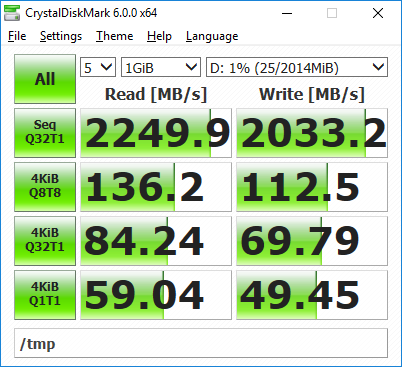
\includegraphics[width=\textwidth]{ramdisk.png}
		\caption{Disk hosted in RAM}
	\end{subfigure}
	\begin{subfigure}[t]{0.45\textwidth}
		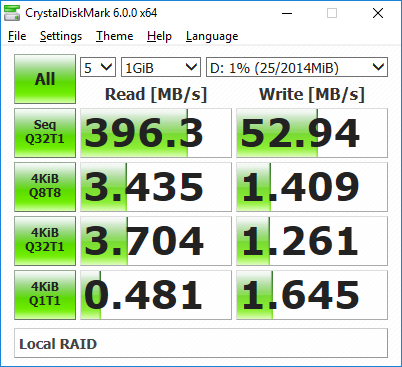
\includegraphics[width=\textwidth]{raid.png}
		\caption{Disk on Local RAID 5}
	\end{subfigure}
	\begin{subfigure}[t]{0.45\textwidth}
		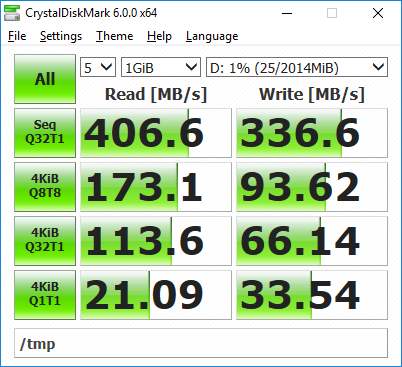
\includegraphics[width=\textwidth]{tmp.png}
		\caption{Disk in /tmp}
	\end{subfigure}
	\begin{subfigure}[t]{0.45\textwidth}
		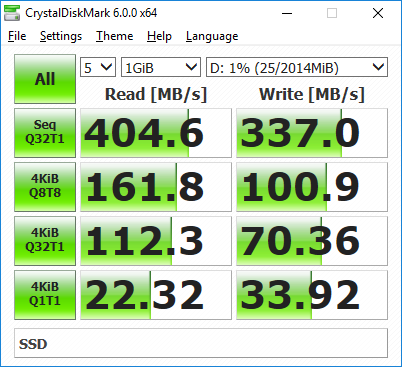
\includegraphics[width=\textwidth]{ssd.png}
		\caption{Disk on main SSD}
	\end{subfigure}
	\begin{subfigure}[t]{0.45\textwidth}
		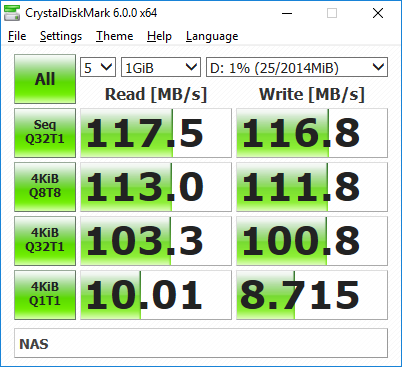
\includegraphics[width=\textwidth]{nas.png}
		\caption{Disk on Network Storage}
	\end{subfigure}
	\caption{Disk Performance tests of Various Kinds}
	\label{fig:disk_performance}
\end{figure}

So, I just want to list the problems I had getting the tests to work.
All the disks had issues with being cached into RAM by default all files under linux are cached into free RAM to improve burst writes and all reads.
It luckily was as easy as changing a drop-down menu in the GUI manager I have to get the "none" cache mode.
The second problem was the hard one to fix.
The disk I made on the NAS was throwing an error in the hypervisor about not being able to lock the file.
After I spent an hour of changing settings, doing research, even changing which protocall was used to mount the network share, it finally would let the VM boot.
Luckily I got all the tests I wanted done and screenshots taken.

\clearpage
Here are some conclusions that I can draw now that the tests are done.
\begin{itemize}
	\item The most obvious is the run-away winner being RAM.
	While it is no surprise that it is fast, I find it interesting how much it still was crippled in the random reads and writes.
	\item The next row has the /tmp and SSD benchmarks where I think the /tmp disk was just shoved onto the SSD.
	The SSD did quite well and shows just how good the performance of these devices are.
	The random reads and writes are very intriguing; two of those read tests make it \textit{faster} than RAM and two of the write tests are on par.
	\item The local RAID 5 is something I find very disapointing.
	I always thought it was faster than that, consiting of all those disks.
	I suppose a harddrive is only so good and the random reads and writes were just asking for too small of sectors to really use the array.
	It is good to note that it is as fast as my SSD when doing sequential reads.
	\item The NAS, the thing I was most interested in, is interesting.
	It has the issue of latency of the network to get in its way, as well as a whole second operating system layer it goes through.
	Even with that, it manages to hold pace with the SSD for the random reads and write.
	The sequential read and write test is at the saturation speed of the network, but it is interesting at how it out performs my local RAID.
	The remote RAID does have 8 disks so perhaps it simply is being twice as fast as my local array.
\end{itemize}

There is a last variable I have not been able to hold down for the NAS test.
For the lcoal machine, I was able to figure out how to turn off caching, but for the NAS machine, I did not know how to do that without disabling it on the whole disk.
Since it is a fairly major thing to just turn off, I decided to just leave it in the condition I was actually going to use it, aka with remote caching enabled.

\section{Passing Hardware Through}

VMs are great and all, but sometimes there is just something more you want a VM to do that requires direct hardware access.
This can include things like special packet filtering using hardware in a NIC or proper full acceleration of some workloads with a GPU.
This realm of cases would typically necessitate giving bare metal access to a system which means it can't be virtualized.
Lately a new technology has come out for PCIe called ACS.
This is a security and safety feature that allows paths to individual hardware on the bus to be isolated from the other hardware.

With ACS and a little footwork on the kernel to expose the functionality, a single process can be given full control over a single PCIe path.
Anything in the path on the bus is handed to the process in charge.
This functionality was first rolled out in Xeon processors as an enterprise level feature, but starting with the 5th generation desktop parts, it has been added to the consumer also.
This feature unfortuanantly is still dependent on the motherboard manufactures to support properly splitting up the paths on the board.

So what does this actually do for VMs?
Lets take the example of that high-end NIC with features to do special things if given proper access to it.
The hypervisor is not focused on whatever special case this card can do, so does not have the features built in already.
What can be done is tell the hypervisor to given exclusive access of that card over to one of the running VMs.
From the perspective of the VM, it simply sees an extra piece of hardware show up, same as if you added an extra core or new harddrive to it.
But now the VM can load up the special sauce drivers and do what it needs to take advantage of the hardware!
The only downside is that the hypervisor can only hand it to a single VM at a time and can not use the hardware itself while it is handed off.

So lets take an example look at passing a GPU to a VM on my desktop (using linux, sorry).
The first step is to enable IOMMU groups on your system.
That might involve recompiling the kernel and is different per distro, but in the kernel config menu you can press "/" at any time and search for \textit{IOMMU}.
This part might not even be neccesary as it probably is already turned on for major distros.

The second step is to hope your manufacturer was nice about chosing PCI bridges that support downstream ACS.
There is a script on the Arch wiki that asks the kernel for what hardware is in what group.\cite{wiki_arch_ovmf}
In fig\ref{fig:iommu_output} I ran the script and shows all my groups.
If you see group 12, it has several items put together in it, which means they are not fully seperated from each other.
This matters because in order to pass 1 thing to a VM, you must pass EVERY item in the same group to the VM.

\begin{figure}[ht]
	\scriptsize
	\begin{verbatim}
	IOMMU Group 0 00:00.0 Host bridge: 4th Gen Core Processor DRAM Controller [8086:0c00]
	IOMMU Group 1 00:01.0 PCI bridge: Xeon E3-1200 v3/4th Gen Core Processor PCI Express x16 Controller [8086:0c01]
	IOMMU Group 2 00:01.1 PCI bridge: Xeon E3-1200 v3/4th Gen Core Processor PCI Express x8 Controller [8086:0c05]
	IOMMU Group 3 00:14.0 USB controller: 8 Series/C220 Series Chipset Family USB xHCI [8086:8c31]
	IOMMU Group 4 00:16.0 Communication controller: 8 Series/C220 Series Chipset Family MEI Controller #1 [8086:8c3a]
	IOMMU Group 5 00:19.0 Ethernet controller: Ethernet Connection I217-V [8086:153b]
	IOMMU Group 6 00:1a.0 USB controller: 8 Series/C220 Series Chipset Family USB EHCI #2 [8086:8c2d]
	IOMMU Group 7 00:1b.0 Audio device: 8 Series/C220 Series Chipset High Definition Audio Controller [8086:8c20]
	IOMMU Group 8 00:1c.0 PCI bridge: 8 Series/C220 Series Chipset Family PCI Express Root Port #1 [8086:8c10]
	IOMMU Group 9 00:1c.2 PCI bridge: 8 Series/C220 Series Chipset Family PCI Express Root Port #3 [8086:8c14]
	IOMMU Group 10 00:1c.5 PCI bridge: 8 Series/C220 Series Chipset Family PCI Express Root Port #6 [8086:8c1a]
	IOMMU Group 11 00:1d.0 USB controller: 8 Series/C220 Series Chipset Family USB EHCI \#1 [8086:8c26]
	IOMMU Group 12 00:1f.0 ISA bridge: Z87 Express LPC Controller [8086:8c44]
	IOMMU Group 12 00:1f.2 SATA controller: 8 Series/C220 Series Chipset Family 6-port SATA Controller 1 [AHCI mode] [8086:8c02]
	IOMMU Group 12 00:1f.3 SMBus: 8 Series/C220 Series Chipset Family SMBus Controller [8086:8c22]
	IOMMU Group 13 01:00.0 VGA compatible controller: NVIDIA Corporation GM204 [GeForce GTX 970] [10de:13c2]
	IOMMU Group 13 01:00.1 Audio device: NVIDIA Corporation GM204 High Definition Audio Controller [10de:0fbb]
	IOMMU Group 14 02:00.0 VGA compatible controller: NVIDIA Corporation GM206 [GeForce GTX 960] [10de:1401]
	IOMMU Group 14 02:00.1 Audio device: NVIDIA Corporation Device [10de:0fba]
	IOMMU Group 15 04:00.0 SATA controller: ASMedia Technology Inc. ASM1062 Serial ATA Controller [1b21:0612]
	IOMMU Group 16 05:00.0 USB controller: NEC Corporation uPD720200 USB 3.0 Host Controller [1033:0194]
	\end{verbatim}
	\vspace{-20pt}
	\caption{IOMMU Groupings on my Desktop}
	\label{fig:iommu_output}
\end{figure}

So you can see that the NVIDIA cards are there, and even tells us which cards are in my system.
I have two cards currently plugged in, a 970 and a 960.
I want to pass only my 960 to a VM, so checking the groups, it says it is in \#14 with some audio device with it.
In order to pass it, we must bind the PCI device to the special VFIO driver when the system boots.
We need to know the PCI device IDs which are given at the end of the lines (so [10de:1401] and [10de:0fba]).
To do this, we will edit the file \underline{/etc/default/grub} and change the line below to include the given options.
If there are things already there, keep them and just add these options after them.

\vspace{-10pt}
\begin{figure}[ht]
	\centering
	\begin{minted}{bash}
		sudo nano /etc/default/grub
	\end{minted}
	\vspace{-20pt}
	\begin{minted}{bash}
		GRUB_CMDLINE_LINUX="intel_iommu=on vfio-pci.ids=10de:1401,10de:0fba"
	\end{minted}
	\vspace{-20pt}
	\begin{minted}{bash}
		sudo grub-config -o /boot/grub/grub.cfg
	\end{minted}
	\vspace{-20pt}
	\caption{Grub Command Line for Boot}
	\label{fig:grub_cmdline}
\end{figure}

\vspace{-10pt}
So after a reboot to get the drivers worked out for the PCI cards, we can now try passing to the VM.
I only know how to do it with KVM but I have heard it was possible to do with other hypervisors.
Lets first make sure you have all the right VM bits installed with the single bash line below.
This will make sure that the backend for virtualising as well as the GUI front end is installed.

\begin{figure}[ht]
	\centering
	\begin{minted}{bash}
		sudo apt install qemu-kvm libvirt-bin ubuntu-vm-builder bridge-utils ovmf
		sudo adduser `id -un` libvirtd
	\end{minted}
	\vspace{-20pt}
	\caption{KVM Install on Ubuntu \cite{wiki_ubuntu_kvm}}
	\label{fig:ubuntu_kvm_install}
\end{figure}

\vspace{-15pt}
After one last reboot, we can now open up virt-manager.
So with our GUI open, we can go through the normal stuff of making a VM with some highlights in fig\ref{fig:kvm_gui}.
The top left of the GUI has the button to make a new VM, where it brings up a window with different options.
Go through the window and fill out settings like you normally would, but make sure to click the \textit{customize} option before clicking finish.
The window after that is where you need to change the firmware used to UEFI so that it plays nicely with the PCI device.
From here you can also add the hardware, which is a rather straight forward affair.
Just make sure to add all devices that are in the same IOMMU group that was listed before.

\begin{figure}[ht]
	\centering
	\begin{subfigure}[t]{0.4\textwidth}
		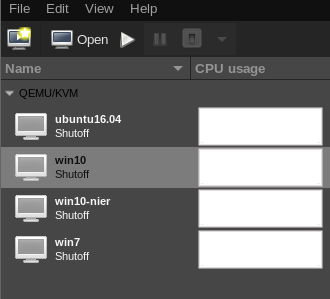
\includegraphics[width=\textwidth]{kvm_main.png}
		\caption{Main GUI}
	\end{subfigure}
	\begin{subfigure}[t]{0.4\textwidth}
		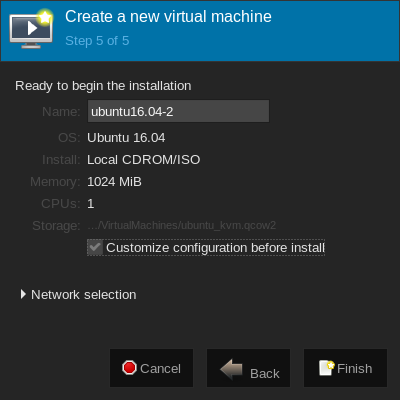
\includegraphics[width=\textwidth]{kvm_custom.png}
		\caption{Check the option to customize}
	\end{subfigure}
	\begin{subfigure}[t]{0.4\textwidth}
		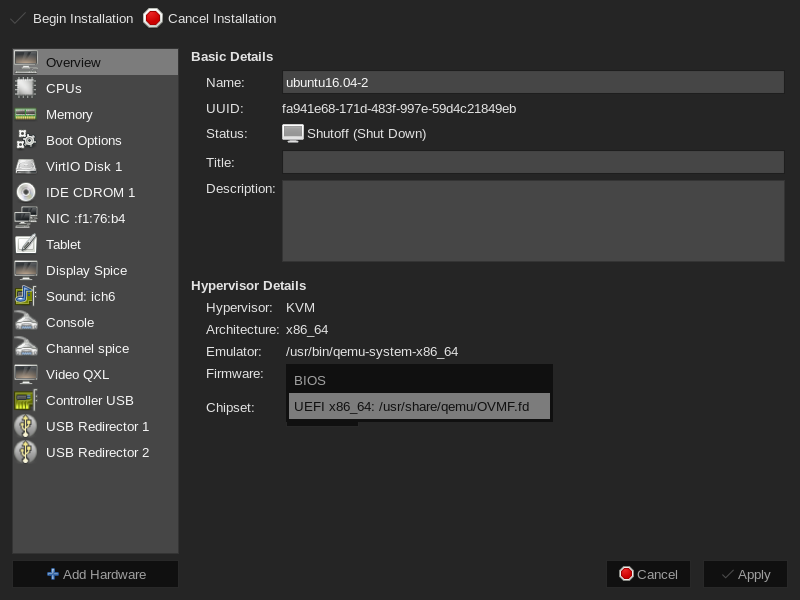
\includegraphics[width=\textwidth]{kvm_uefi.png}
		\caption{Change the firmware to UEFI}
	\end{subfigure}
	\begin{subfigure}[t]{0.4\textwidth}
		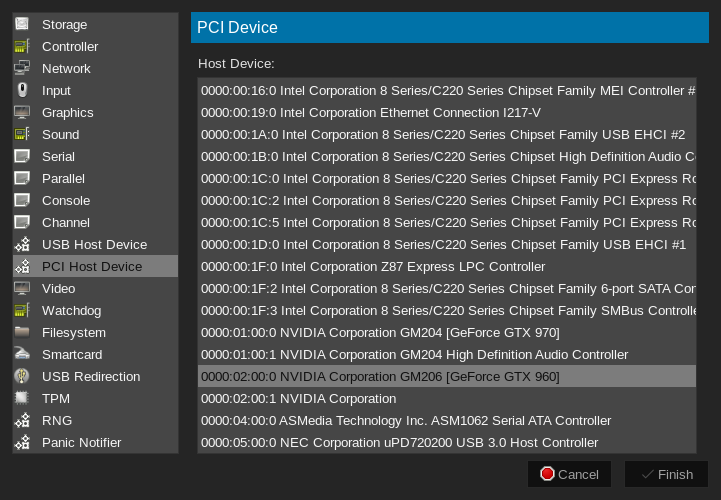
\includegraphics[width=\textwidth]{kvm_pcie.png}
		\caption{Adding a new PCI device}
	\end{subfigure}
	\caption{Highlights of making a new VM with hardware attached}
	\label{fig:kvm_gui}
\end{figure}

So now that you have the VM, you can go through the install process and get a working system.
Assuming you just installed windows, you can open up device manager and see it there.
But alas, NVidia is annoying in that they artifically hold the cards hostage and try to get you to buy a quadro brand.
The device under device manager (windows) has an error code 43 after you just got the drivers installed.

\begin{figure}[ht]
	\centering
	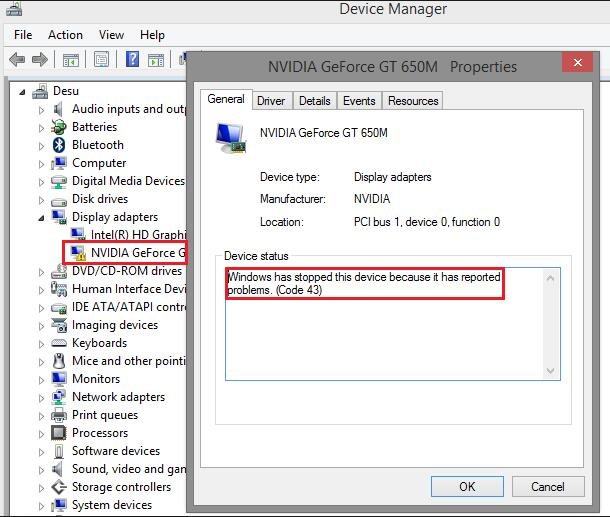
\includegraphics[width=0.8\textwidth]{error_43.jpg}
	\caption{Example Image of code 43 \cite{image_code43}}
\end{figure}

In order for this to work, you have to edit the config file of the VM directly.
Simply make the changes in fig\ref{fig:config_edit} (thanks to arch wiki again \cite{wiki_arch_ovmf}).
If the tag does not already exist, feel free to add it at the right location.

\begin{figure}[ht]
	\centering
	\small
	\begin{minted}{bash}
		virsh edit [VM name]
	\end{minted}
	\begin{minted}{xml}
		<features>
			<hyperv>
				...
				<vendor_id state='on' value='123456789ab'/>
				...
			</hyperv>
			...
			<kvm>
				<hidden state='on'/>
			</kvm>
		</features>
	\end{minted}
	\vspace{-15pt}
	\caption{Config Changes to Stop Error 43}
	\label{fig:config_edit}
\end{figure}

And with that all done, booting the VM should now have the drivers happy and let you do serious work such as CAD or Video Games at full accelerated speed.
There is a single drawback with having the hypervisor hide itself, the VirtIO devices will not work.
Those devices lets the guest take shortcuts for sake of performance because the guest knows it is in a VM.
That is not a big deal, seems only to be about a small hit on my system.

So just a few minor notes about passing PCI devices.
I went through the steps of doing an NVidia card, as that is what I have and is the majority.
NVidia cards, when they work, work well and bug free.
AMD cards through have a known problem of not propperly resetting when a VM shutsdown.
If you pass an AMD card, and you need to reboot the VM, then you must also reboot the host to reset the card.
But, AMD does not require that you hide the VM and so are less hostile to users.

Last major note is my processor in terms of ACS support.
My CPU is a 4th generation, which is before they started putting support in at all.
Recall that I said ACS allows this to work, and while by default it is true, you can get around needing it.
To get around this, I have to patch my kernel to pretend there is ACS support.
This is dangerous as it is an escape route out of the VM to the host.
It can also cause system instability as it assumes a PCI path will not interfere with other things when it very well might.
I have not noticed any problems with many hours of runtime, but it is not running as intended and so no guarantees.

%------------------------------------------------------------------------------------------------------------------------------------------------
\clearpage
\newpage
\begin{thebibliography}{9}

\bibitem{wiki_raidLevels}
	En.wikipedia.org. (2018). Standard RAID levels. [online] Available at: https://en.wikipedia.org/wiki/Standard\_RAID\_levels [Accessed 25 Jan. 2018].

\bibitem{wiki_arch_ovmf}
	Wiki.archlinux.org. (2018). PCI passthrough via OVMF - ArchWiki. [online] Available at: https://wiki.archlinux.org/index.php/PCI\_passthrough\_via\_OVMF [Accessed 26 Jan. 2018].

\bibitem{wiki_ubuntu_kvm}
	Help.ubuntu.com. (2018). KVM/Installation - Community Help Wiki. [online] Available at: https://help.ubuntu.com/community/KVM/Installation [Accessed 26 Jan. 2018].

\bibitem{image_code43}
	Driverdr.com. (2018). Solve code 43 with NVida Drivers. [online] Available at: https://www.driverdr.com/windows10/images/3-ways-to-solve-nvidia-driver-error-code-43-windows-10/graphic-driver-code-43-error.jpg [Accessed 26 Jan. 2018].

\end{thebibliography}

\end{document}